\chapter{Random Boolean Networks}\label{rbn}
\lhead[\fancyplain{}{\bfseries\thepage}]{\fancyplain{}{\bfseries\rightmark}}


In this chapter we explain the basic concepts of Random Boolean Network proposed for the first time by Kauffman.

\section{Random Boolean Networks}
Random Boolean networks (RBNs) were introduced in
1969 by S. Kauffman as a simple model of genetic systems.
Each gene was represented by a node
that has two possible states, “on” (corresponding to a
gene that is being transcribed) and “off” (corresponding
to a gene that is not being transcribed). There are altogether N nodes, and each node receives input from K
randomly chosen nodes, which represent the genes that
control the considered gene. Furthermore, each node is
assigned an update function that prescribes the state of
the node in the next time step, given the state of its input nodes. This update function is chosen from the set
of all possible update functions according to some probability distribution. Starting from some initial configuration, the states of all nodes of the network are updated
in parallel. Since configuration space is finite and since
dynamics is deterministic, the system must eventually return to a configuration that it has had before, and from
then on it repeats the same sequence of configurations
periodically: it is on an attractor.

\section{The model}
Let's consider a network of $N$ nodes. The state of each node at a time $t$ is given by $\sigma_i(t) \in {0,1}$ with $ i = 1,...,N$.
The $N$ nodes of the network can therefore together assume $2^N$ different states.
The number of incoming links to each node $i$  is denoted by $k_i$ and is drawn
randomly independently from the distribution $P(k_i)$.
The dynamical state of each $\sigma_i(t)$ is updated synchronously by a Boolean function $\Lambda_i$:
$$
\Lambda_i:\{0,1\}^{k_i} \to \{0,1\}
$$ 
An update function specifies
the state of a node in the next time step, given the state
of its $K$ inputs at the present time step. Since each of the
$K$ inputs of a node can be on or off, there are $M = 2^K$ possible input states.
The update function has to specify the new state of a node for each of these input states.
Consequently, there are $2^M$ different update functions.
For example let's consider a network with $K=1$, so all the functions $\Lambda_i$ receives the input from one single node. 
In general each element 
receives inputs from exactly $K$ nodes, so we have a dynamical system defined from:

\begin{equation}
\sigma_i(t+1)=\Lambda_i(\sigma_{i_1}(t),\sigma_{i_2}(t), ...,\sigma_{i_K}(t)).
\end{equation}  

So, the randomness of these network appears at two levels: in the connectivity of the network (which node is linked
to which) and the dynamics (which function is attributed to which node).

\section{Topology}
For a given number $N$ of nodes and a given number
$K$ of inputs per node, a RBN is constructed by choosing
the $K$ inputs of each node at random among all nodes.
If we construct a sufficiently large number of networks in
this way, we generate an ensemble of networks. In this
ensemble, all possible topologies occur, but their statis-
tical weights are usually different. Let us consider the
simplest possible example, $N = 2$ and $K = 1$, shown
in Figure~\ref{fig:rb}. There are 3 possible topologies.



\begin{figure}[h]
\centering
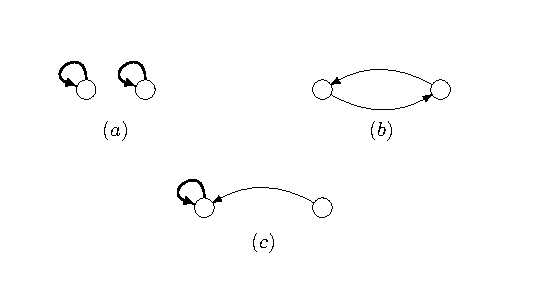
\includegraphics[scale=1]{figurenetworks.pdf}
\caption{Set of all possible networks with $N=2$ and $K=1$.}
\label{fig:rb}
\end{figure}

Topologies (a) and (b) have each the statistical weight $1/4$ in
the ensemble, since each of the links is connected in the
given way with probability $1/2$. Topology (c) has the
weight $1/2$, since there are two possibilities for realizing
this topology: either of the two nodes can be the one
with the self-link.


While the number of inputs of each node is fixed by
the parameter $K$, the number of outputs (i.e. of outgo-
ing links) varies between the nodes. The mean number of
outputs must be $K$, since there must be in total the same
number of outputs as inputs. A given node becomes the
input of each of the N nodes with probability $\frac{K}{N}$ . In
the thermodynamic limit $N \to \infty$ the probability distribution of the number of outputs is therefore a Poisson
distribution:

$$
P_{out}(k) = \frac{K^k}{k!}e^{-K}
$$

\section{Dynamics}

All nodes are updated at the same time
according to the state of their inputs and to their update
function. Starting from some initial state, the network
performs a trajectory in state space and eventually arrives on an \emph{attractor}, where the same sequence of states
is periodically repeated. Since the update rule is deterministic, the same state must always be followed by the
same next state. If we represent the network states by
points in the $2^N$-dimensional state space, each of these
points has exactly one “output”, which is the successor
state. We thus obtain a graph in state space.
The size or length of an attractor is the number of
different states on the attractor. The basin of attraction
of an attractor is the set of all states that eventually
end up on this attractor, including the attractor states
themselves. The size of the basin of attraction is the
number of states belonging to it. The graph of states
in state space consists of unconnected components, each
of them being a basin of attraction and containing an
attractor, which is a loop in state space. The transient
states are those that do not lie on an attractor. They are
on trees leading to the attractors.


Let us illustrate these concepts by studying the small
$K = 1$ network shown in Figure~\ref{fig:rb2}, which consists of 4
nodes:

\begin{figure}[h]
\centering
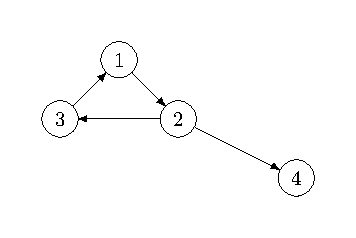
\includegraphics[scale=1]{figurenetworks2.pdf}
\caption{A small network with $N=4$ and $K=1$.}
\label{fig:rb2}
\end{figure}

If we assign to the nodes 1,2,3,4 the functions invert,
invert, copy, copy, an initial state $1111$ evolves in the
following way:

$$
1111 \to 0011 \to 0100 \to 1111
$$

This is an attractor of period 3. If we interpret the bit se-
quence characterizing the state of the network as a number in binary notation, the sequence of states can also be
written as

$$
15 \to 3 \to 4 \to 15
$$

The entire state space is shown in Figure~\ref{fig:rb3}:
\begin{figure}[h]
\centering
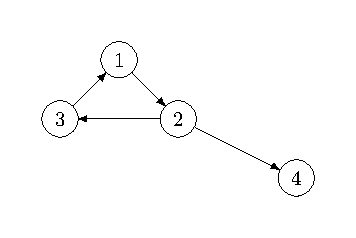
\includegraphics[scale=1]{figurenetworks2.pdf}
\caption{The state space of the network shown in Figure~\ref{fig:rb2}, if
the functions copy, copy, invert, invert are assigned to the four
nodes. The numbers in the squares represent states, and ar-
rows indicate the successor of each state. States on attractors
are shaded.}
\label{fig:rb3}
\end{figure}

There are 4 attractors, two of which are fixed points
(i.e., attractors of length 1). The sizes of the basins of
attraction of the 4 attractors are 6,6,2,2. If the function
of node 1 is a constant function, fixing the value of the
node at 1, the state of this node fixes the rest of the
network, and there is only one attractor, which is a fixed
point. Its basin of attraction is of size 16. If the functions
of the other nodes remain unchanged, the state space
then looks as shown in Figure~\ref{fig:rb4}

\begin{figure}[h]
\centering
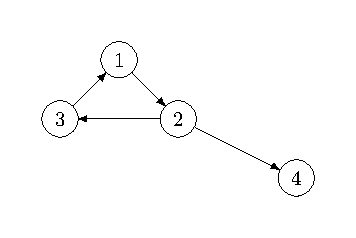
\includegraphics[scale=1]{figurenetworks2.pdf}
\caption{The state space of the network shown in Figure~\ref{fig:rb2},
if the functions 1, copy, invert, invert are assigned to the four
nodes.}
\label{fig:rb4}
\end{figure}

Before we continue, we have to make the definition of
attractor more precise: as the name says, an attractor
“attracts” states to itself. A periodic sequence of states
(which we also call cycle) is an attractor if there are states
outside the attractor that lead to it. However, some netaworks contain cycles that cannot be reached from any
state that is not part of it. For instance, if we removed
node 4 from the network shown in Figure 2.2, the state
space would only contain the cycles shown in Figure 2 C,
and not the 8 states leading to the cycles. In the follow-
ing, we will use the word “cycle” whenever we cannot be
confident that the cycle is an attractor.


\section{Applications}

Let us now make use of the definitions and concepts
introduced in this section in order to derive some results
concerning cycles in state space. First, we prove that in
an ensemble of networks with update rule 1 (biased functions) or rule 2 (weighted classes), there is on an average
exactly one fixed point per network. A fixed point is a
cycle of length 1. The proof is slightly different for rule
1 and rule 2. Let us first choose rule 2. We make use of
the property that for every update function the inverted
function has the same probability. The inverted function
has all 1s in the output replaced with 0s, and vice versa.
Let us choose a network state, and let us determine for
which fraction of networks in the ensemble this state is a
fixed point. We choose a network at random, prepare it
in the chosen state, and perform one update step. The
probability that node 1 remains in the same state after
the update, is 1/2, because a network with the inverted
function at node 1 occurs equally often. The same holds
for all other nodes, so that the chosen state is a fixed
point of a given network with probability $2^{−N}$ . This
means that each of the 2 N states is a fixed point in the
proportion $2^{−N}$ of all networks, and therefore the mean
number of fixed points per network is 1. We will see
later that fixed points may be highly clustered: a small
proportion of all networks may have many fixed points,
while the majority of networks have no fixed point.


Next, we consider rule 1. We make now use of the
property that for every update function a function with
any permutation of the input states has the same probability. This means that networks in which state A leads
to state B after one update, and networks in which another state C leads to state B after one update, occur
equally often in the ensemble. Let us choose a network
state with n 1s and $N − n$ 0s. The average number of
states in a network leading to this state after one update
is $2^N p^n (1 − p^{N −n}$ . Now, every state leads equally often
to this state, and therefore this state is a fixed point in
the proportion $p^n (1 − p)^{N−n}$ of all networks. Summation
over all states gives the mean number of fixed points per
network, which is 1.

Finally, we derive a general expression for the mean
number of cycles of length L in networks with $K = 2$
inputs per node. The generalization to other values of $K$
is straightforward. Let $\langle C_L\rangle_N$ denote the mean number
of cycles in state space of length $L$, averaged over the
ensemble of networks of size $N$ . On a cycle of length
L, the state of each node goes through a sequence of
1s and 0s of period L. Let us number the $2^L$ possible
sequences of period L of the state of a node by the index
j, ranging from 0 to $m = 2^L − 1$. Let $n_j$ denote the
number of nodes that have the sequence $j$ on a cycle of
length$ L$, and $(P_L )^j_{l,k}$ the probability that a node that
has the input sequences $l$ and $k$ generates the output
sequence $j$. This probability depends on the probability distribution of update functions.



Then

\begin{equation}
\langle C_L\rangle_N = \frac{1}{L} \sum_{n_j} \frac{N!}{n_0! \dots n_m!} \prod_j \big(\sum_{l,k}\frac{n_ln_k}{N^2}(P_L)^j_{l,k}\big)^{n_j}
\end{equation}

The factor 1/L occurs because any of the L states on the
cycle could be the starting point. The sum is P
over all
possibilities to choose the values {n j } such that j n j =
N . The factor after the sum is the number of different
ways in which the nodes can be divided into groups of the
sizes n 0 , n 1 , n 2 , . . . , n m . The product is the probability
that each node with a sequence j is connected to nodes
with the sequences l and k and has an update function
that yields the output sequence j for the input sequences
l and k. This formula was first given in the beautiful
paper by Samuelsson and Troein [10].

